\documentclass[11pt,letterpaper,boxed]{pset}

\usepackage[margin=0.75in]{geometry}
\usepackage{ulem}

\begin{document}

    \problemlist{PHYS051 HW08}
    \begin{center}
        *E34.26, E34.23, P34.14, E34.17, E34.18
    \end{center}
    
    \begin{problem} [*E34.26]
        A stiff wire bent into a semicircle of radius $a$ is rotated with a frequency $f$ in a uniform magnetic field, as suggested in Fig. 34-51. What are
        \begin{enumerate}
            \item [a.] the frequency and
            \item [b.] the amplitude of the emf induced in the loop?
        \end{enumerate}
    \end{problem}
    
    \begin{figure*} [ht]
        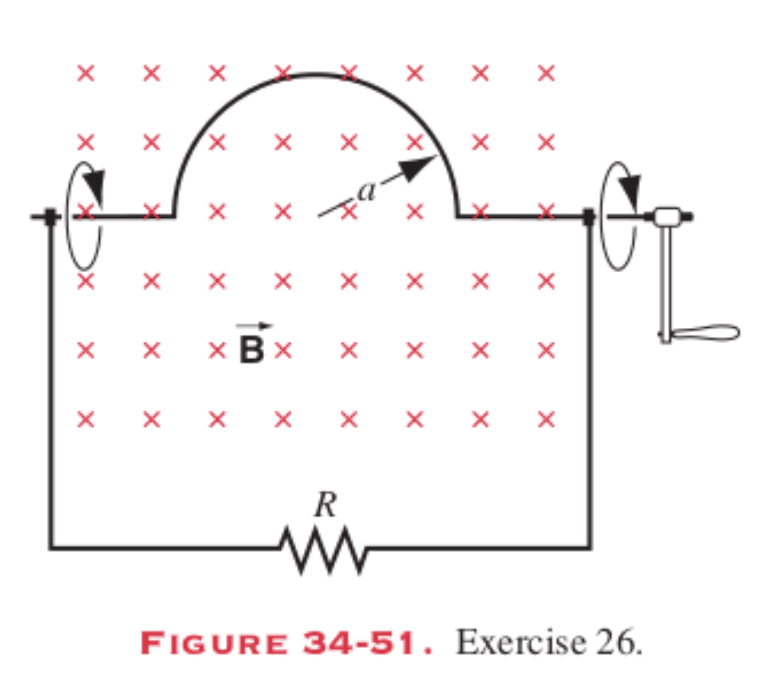
\includegraphics[width=125px]{HW8Images/E34-26.png}
        \label{fig:E34-26}
    \end{figure*}
    \newpage
    
    \begin{problem} [E34.23]
        A rectangular loop of wire with length $a$, width $b$, and resistance $R$ is placed near an infinitely long wire carrying current $i$, as shown in Fig. 34-49. The distance from the long wire to the loop is $D$. Find
        
        \begin{enumerate}
            \item [a.] the magnitude of the magnetic flux through the loop and
            \item [b.] the current in the loop as it moves away from the long wire with speed $v$.
        \end{enumerate}
    \end{problem}
    
    \begin{figure*} [ht]
        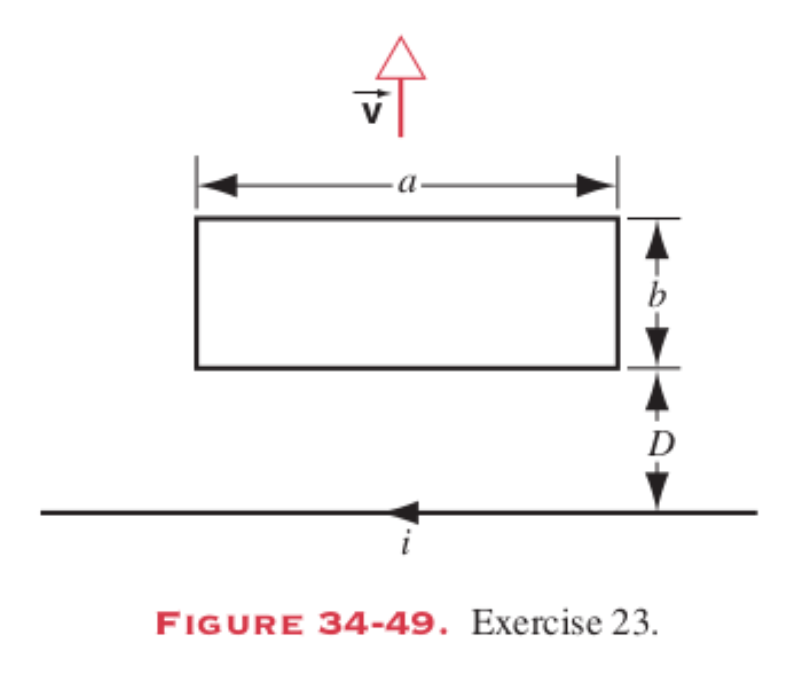
\includegraphics[width=125px]{HW8Images/E34-23.png}
        \label{fig:E34-23}
    \end{figure*}
    \newpage
    
    \begin{problem} [P34.14]
        A uniform magnetic field $\Vec{B}$ fills a cylindrical volume of radius $R$. A metal rod of length $L$ is placed as shown in Fig. 34-63. If $B$ is changing at the rate $dB/dt$, show that the emf that is produced by the changing magnetic field and that acts between the ends of the rod is given by 
        
        \[\mathscr{E} = \frac{dB}{dt} \frac{L}{2} \sqrt{R^2 - (\frac{L}{2})^2}.\]
    \end{problem}
    
    \begin{figure*} [ht]
        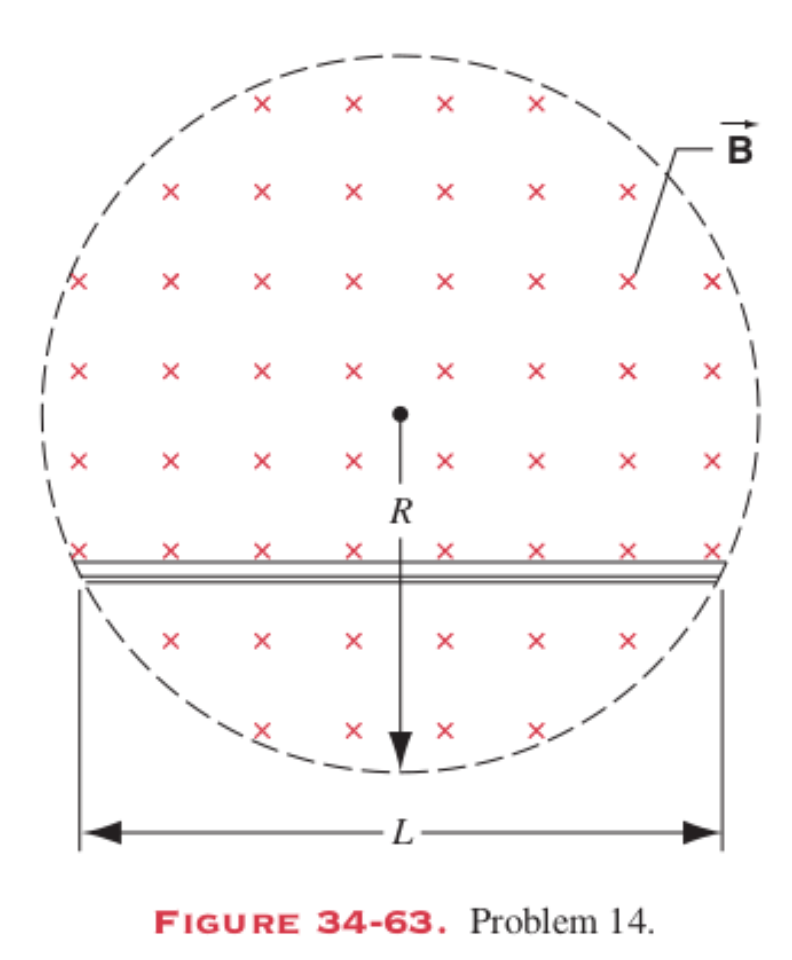
\includegraphics[width=125px]{HW8Images/P34-14.png}
        \label{fig:P34-14}
    \end{figure*}
    \newpage
    
    \begin{problem} [E34.17]
        In Fig. 34-17, a conducting rod of mass $m$ and length $L$ slides without friction on two long, horizontal rails. A uniform vertical magnetic field $\Vec{B}$ fills the region in which the rod is free to move. The generator G supplies a current $i$ that flows down one rail, across the rod, and back to the generator along the other rail. A student monitors the generator, continually adjusting it so that the current it supplies is constant regardless of the load. Find the velocity of the rod as a function of time, assuming it to be at rest at $t = 0$.
    \end{problem}
    
    \begin{figure*} [ht]
        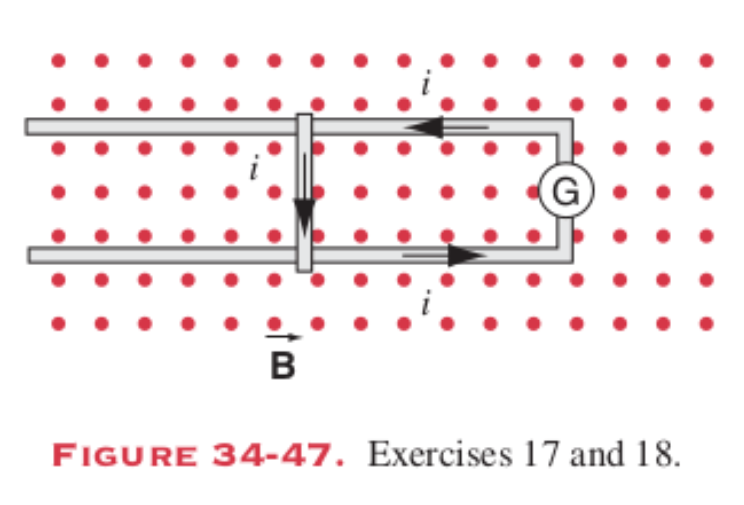
\includegraphics[width=125px]{HW8Images/E34-17-18.png}
        \label{fig:E34-17}
    \end{figure*}
    \newpage
    
    \begin{problem} [E34.18]
        In Exercise 17 (see 34-47) the generator G is replaced by a battery that supplies a constant emf $\mathscr{E}$. 
        
        \begin{enumerate}
            \item [a.] Show that the velocity of the rod now approaches a constant terminal value $\Vec{v}$ and give its magnitude and direction.
            \item [b.] What is the current in the rod when this terminal velocity is reached? 
            \item [c.] Analyze both this situation and that of Exercise 17 from the point of view of energy transfers.
        \end{enumerate}
    \end{problem}
    \begin{figure*} [ht]
        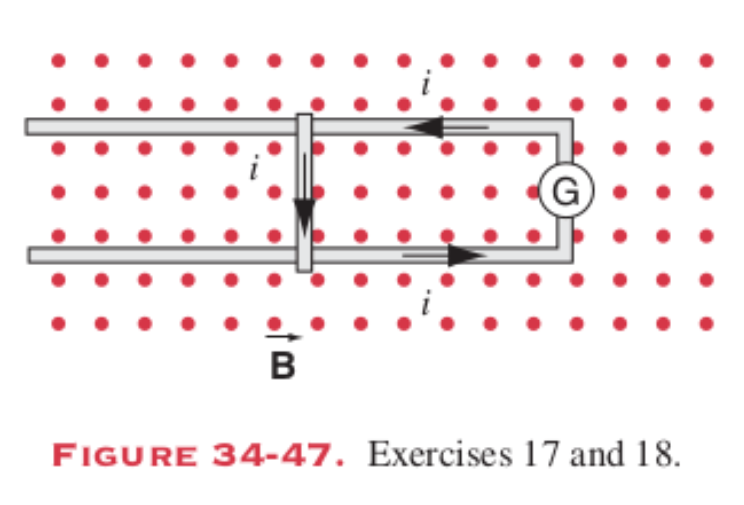
\includegraphics[width=125px]{HW8Images/E34-17-18.png}
        \label{fig:E34-18}
    \end{figure*}
\end{document}